\chapter{Monte Carlo Simulation of an Ideal Gas}

\section{Introduction}

In this lab, we will introduce the Monte Carlo method, an approach to
solving a wide range of problems by repeatedly drawing random numbers.
You will use histograms to compare randomly thrown values to their
corresponding probability distributions functions.  You will construct
a Monte Carlo simulation of a 2-D ideal gas, and show that the
molecular velocities follow the Maxwell-Boltzman distribution.

For a faster but more challenging path, complete only the problems
(including optional challenge problems) in Sections~\ref{sec:mcint},
\ref{sec:mbdist}, and \ref{sec:idealgas}.

\section{Preparation}

In this exercise, we will make use of slicing and boolean masks, which
are covered in sections 1.4.1.5 and 1.4.1.7 of the Scientific Python
lecture notes.  Make sure you are comfortable enough with these
concepts to understand the following exercises:\\

\plot Run the following snippet, and make sure you understand the output:
\begin{python}
x = np.arange(10)
print("x       = ", x)
# all but the first element:
print("x[1:]   = ", x[1:])
# all but the last element:
print("x[:-1]  = ", x[:-1])
# the first 4 elements:
print("x[:4]   = ", x[:4])
# elements from index 2 to 6:
print("x[2:7]  = ", x[2:7])
# elements in reverse order:
print("x[::-1] = ", x[::-1])
\end{python} \vskip 0.25cm

\newpage

\plot Run the following snippet, 
\begin{python}
x = np.arange(5)
print("x =         ", x)
print("midpoints:  ", (x[1:]+x[:-1])/2)
\end{python}
which demonstrates a trick we will be using later, for calculating the
midpoints between each value in \pyth{x}.  Note that the first array
has five entries, the second has four.\\

\plot Run the following snippet, and make sure you understand the output:
\begin{python}
x = np.array([1,2,1,4,5,1,7,3])
print("x       = ", x)
mask = x > 2
print("mask    = ", mask)
print("x[mask] = ", x[mask])
\end{python} \vskip 0.25cm

\plot Run the following snippet, 
\begin{python}
x = np.array([1,2,1,4,5,1,7,3])
mask = x>3
np.sum(mask)
\end{python}
which demonstrates a trick we will using later, for counting the
number of entries in an array which satisfy a particular condition.\\

\section{Generating random numbers}

The Monte Carlo method relies on the generation of random numbers, so
we will start there.  The numbers we generate using computers are
actually ``pseudorandom'' numbers, because they are deterministically
obtained from an algorithm.  However, the algorithm is choosen so that
the numbers appear random for practical purposes.  This is no small
concern.  Much of the computational work in the early 1970's had to be
redone because of the widespread use of a deeply flawed pseudorandom
number generator called RANDU.

In this section, you will generate a pseudorandom number sequence
using the linear congruential method.  This sequence is determined
iteratively from the simple relationship:
\begin{displaymath}
  I_{n+1} = (a \, I_{n} + c) \bmod M
\end{displaymath}
Recall that $x \bmod y$ (coded as \pyth{x % y} in Python) is the
remainder after integer division (\pyth{x//y} in Python).  Each $I_n$
is called a seed, and the initial seed $I_0$ must be provided to start
the sequence.  Notice that the seeds are all integers in the range
from 0 to $(M-1)$.  If we wish to convert these seeds into a random
variable $x$ in the range from 0 to $L$, we simply use $x_n = L * I_n
/ M$.  As long as $M$ is much larger than $L$, $x$ is approximately
continuous.

The algorithm works because the product $a*I_{n}$ is generally many
times larger than $M$, so the remainder is effectively a uniform
random number.  The effectiveness of this algorithm is highly
dependend on the choice of $a$,$c$, and $M$.  Choose poorly and you get
RANDU.  Choose wisely and you get the highly regarded algorithm of
Park and Miller.  We will do the latter and use $a=7^5$, $c=0$, and $M
= 2^{31}-1$.\\

\plot Define a function:
\begin{python}
  def parkmiller(i):
      # your code here
      return i # updated value
\end{python}
which, given a seed i, returns the next seed in the Park and Miller
algorithm.  Check your code by testing that for a initial seed of one,
the generator returns a {\bf seed} of 1043618065 after 10000 calls.\\

\plot Use your \pyth{parkmiller(i)} function to fill a numpy array
\pyth{xarr} with 5 randomly thrown $x$ values in the range $[0,1]$.  Check you
code with:
\begin{python}
  print(np.around(xarr,2))
\end{python} \vskip 0.25cm

Now that we have seen how randomly number are generated, we will use the standard numpy tool to produce array of randomly drawn values as needed for us:\\

\plot Use the \pyth{np.random.uniform} to create an array \pyth{xarr}
of five randomly thrown $x$ values in the range $[0,1]$.  Check you
code with:
\begin{python}
  print(np.around(xarr,2))
\end{python}

\section{Probability Density Functions and Histograms}

\begin{figure}[htbp]
\begin{center}
{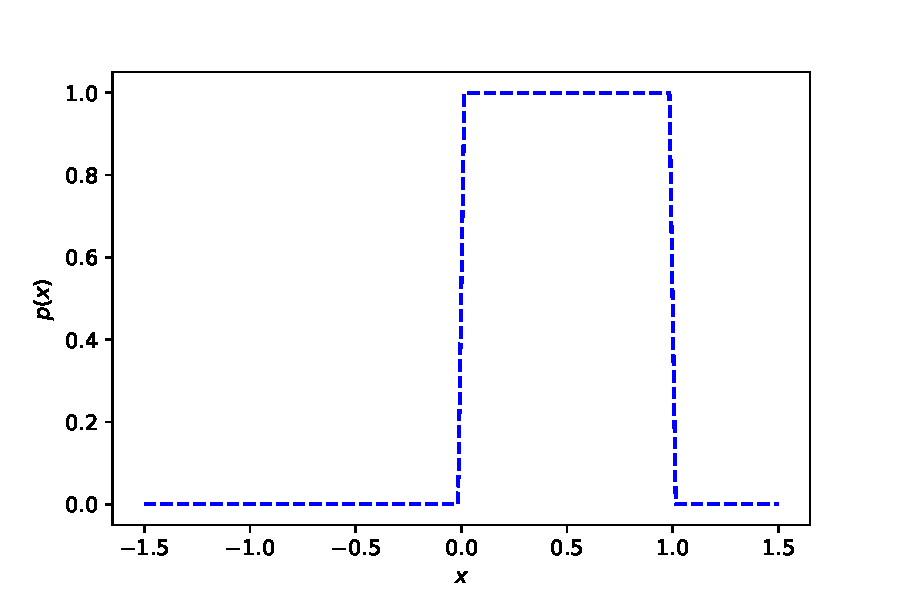
\includegraphics[width=0.45\textwidth]{figs/hist/flatpdf.pdf}}
\end{center}
\caption{\label{fig:flatpdf} The PDF for the process of throwing a
  random variable uniformly in the region $[0,1]$.}
\end{figure}

\noindent
When I generate ten random numbers from the Park and Miller algorithm, I get
the following ten values:
\begin{verbatim}
[0.6448101  0.32334154 0.40125851 0.95175061 0.07252577 0.94062374
 0.06316977 0.69433175 0.63370098 0.61235022]
\end{verbatim}
We say that these ten numbers are thrown (like dice) or drawn (like
cards?) uniformly in the interval from $[0,1]$.  How can we describe
this process of thowing random numbers in terms of probability?  The
probability of drawing a particular number, like 0.06316977 is
extremely small.  If the computer had unlimited precision, the
probability of drawing any particular number would drop all the way to
zero.  Probability by itself doesn't seem to be very useful here.  The
solution is to recognize that it is the probability of throwing a number in
some region $[a,b]$ which is non-zero.  Instead of a probality, we describe
this process by a probability density function (PDF), in this case:
\begin{equation}
  \label{eqn:flatpdf}
  p(x) =
  \begin{cases}
    1 & 0 \leq x \leq 1 \\
    0 & {\rm otherwise} \\
  \end{cases} 
\end{equation}
This PDF is illustrated in Fig.~\ref{fig:flatpdf}.  To find the probability $P$ that we would throw $x$ in some interval $[a,b]$, we integrate the probability density function:
\begin{displaymath}
  P = \int_a^b p(x) \, dx
\end{displaymath}
For example, the probability that we throw a number less than one half is:
\begin{displaymath}
  P = \int_{-\infty}^\frac{1}{2} p(x) \, dx = \int_{0}^\frac{1}{2} 1 \, dx = \frac{1}{2} 
\end{displaymath}
As are all PDFs, this one is normalized to a total probability of one:
\begin{displaymath}
  \int_{-\infty}^{+\infty} p(x) \, dx = \int_0^1 1 \, dx = 1
\end{displaymath}\\

\plot Define a python function:
\begin{python}
  def pdf(x):
      # your code here
      return p
\end{python}
which implements the PDF from Equation~\ref{eqn:flatpdf}.  Use it to create $x$ and $y$ values for plotting as:
\begin{python}
  xf = np.linspace(-1.5,1.5,100)
  yf = pdf(xf)
\end{python}
Reproduce the plot in Fig.~\ref{fig:flatpdf}.  Hint: for this to work,
you have to make sure the function \pyth{pdf(x)} can handle properly
the case that x is a numpy array, and return a numpy array of the same
size.\\

But how can we be verify that our numbers drawn from the Park and Miller algorithm:
\begin{verbatim}
[0.6448101  0.32334154 0.40125851 0.95175061 0.07252577 0.94062374
 0.06316977 0.69433175 0.63370098 0.61235022]
\end{verbatim}
are actually being drawn from the PDF in Fig.~\ref{fig:flatpdf}?  The
tool of choice for seeing the ``shape'' of a list of values is the
histogram, and the process of building one is illustruated in
Fig.~\ref{fig:histeg}.  First, let's draw 1000 random values.  One way
to visualize these values is shown in Fig.~\ref{fig:histeg}a, which
simply plots each value above the throw number (from 0 to 1000).  To
build a histogram, we devide the $x$ range into small regions, called
{\em bins}.  For example, we have a bin from 0.25 to 0.5, as indicated
by the dashed red lines.  The number of blue points contained within
that range is 237.  In Fig.~\ref{fig:histeg}b, we plot the count as
the red point.  The $y$-value of the point is the count 237.  The
$x$-value is the middle of the bin:
\begin{displaymath}
(0.50+0.25)/2 = 0.375
\end{displaymath}
We continue this process for as many bins as we wish to plot.  The
result is the entire set of points in Fig.~\ref{fig:histeg}b which we
call a histogram.  A histogram is a set of bins, with a count
corresponding to each bin.

\begin{figure}[htbp]
\begin{center}
\begin{tabular}{cc}
{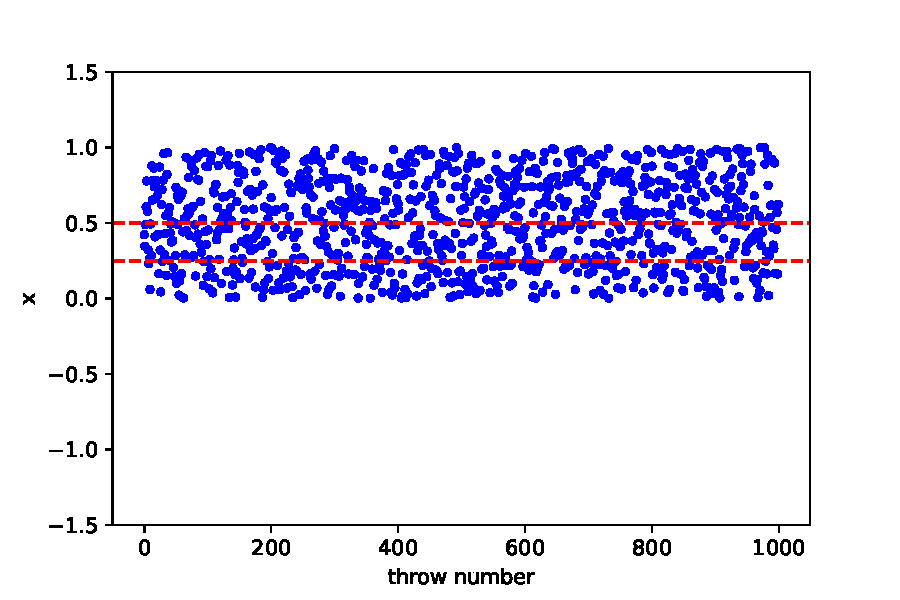
\includegraphics[width=0.45\textwidth]{figs/hist/throwflat.pdf}} &
{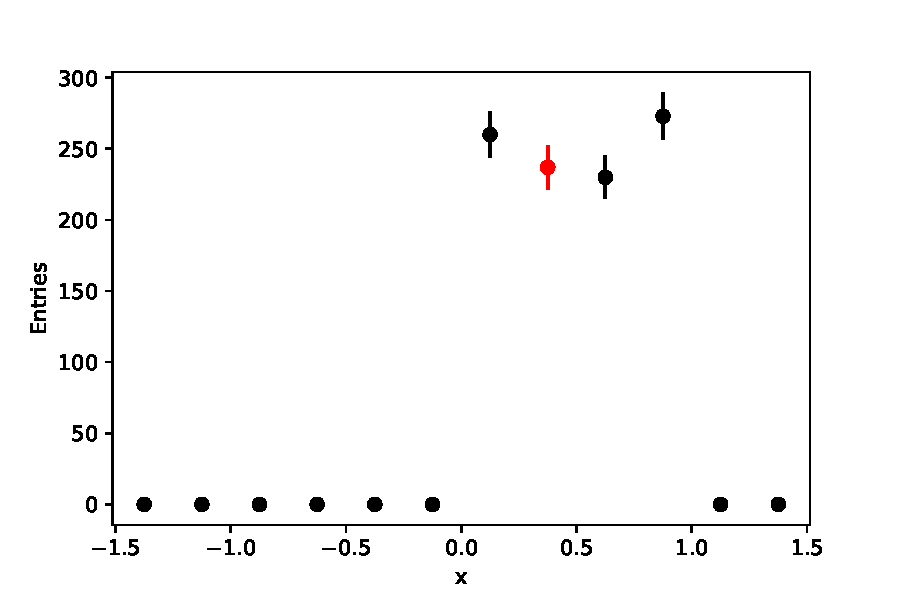
\includegraphics[width=0.45\textwidth]{figs/hist/flathist.pdf}} \\
(a) & (b) \\
\end{tabular}
\end{center}
\caption{\label{fig:histeg} The 1000 measurements of variable $x$ in (a) are used to produce the histogram in (b).  The red data point in (b) is the count of the number of entries in range indicated by the red dashed lines in (a).}
\end{figure}

Notice that each data point in our histogram has an error bar: the
verticle line passing through each point in the histogram.  A
fundamental result from statistics is that the best estimate for the
statistical uncertainty on a count $N$ of independent occurances is
simply $\sqrt{N}$.  The error bars in Fig.~\ref{fig:histeg}b have been
taken as the square root of the count in each bin.

Fortunately, the process of calculating a histogram from an array of values is handled by the python function \pyth{np.histogram}, which you will use in the following exercise:\\

\plot Run the following code snippet:
\begin{python}
NTOT = 1000  # total number of events thrown
NBIN = 12    # number of bins in histogram
XMIN = -1.5  # maximum X value
XMAX = 1.5   # minimum X value
# throw NTOT random values uniformly in [0,1]:
xarr = np.random.uniform(size=NTOT)
#create a histogram from the random values in xarr:
# hx:   the histogram counts (length NBIN)
# edges: the bin edges (length NBIN+1)
hx,edges = np.histogram(xarr,bins=NBIN,range=(XMIN,XMAX))
# calculate the center of each bin, for plotting:
cbins = (edges[1:]+edges[:-1])/2
# calculate the error in each bin as the square root of the count
err   = hx**0.5
# plot the histogram, including errorbars, using the errorbar function:
plt.errorbar(cbins,hx,yerr=err,fmt="ko",label="Histogram")
# add the labels
plt.xlabel("x")
plt.ylabel("Entries")
\end{python}
to construct a histogram like that of Fig.~\ref{fig:histeg}b.\\

There are some lines of particular importance in the code snippet,
which you will need to understand to succeed in this lab.  This line:
\begin{python}
hx,edges = np.histogram(xarr,bins=NBIN,range=(XMIN,XMAX))
\end{python}
actually creates the histogram for the array \pyth{xarr}.  It creates
\pyth{NBIN=12} bins in range from \pyth{XMIN=-1.5} to \pyth{XMAX=1.5}.
The count for each bin is contained in the array \pyth{hx} which has length \pyth{NBIN}.  The edges of the bins are contained in the array \pyth{bins} which has length \pyth{NBIN+1}. Because they are different lengths, you cannot simply plot \pyth{hx} versus \pyth{bins}.  Instead, we calculate the bin centers with the line:
\begin{python}
cbins = (edges[1:]+edges[:-1])/2
\end{python}
which uses slicing to produce an array of length \pyth{NBIN}
containing the bin centers.
We calculate the statistical error for each point in the histogram as the square root of the count:
\begin{python}
err   = hx**0.5
\end{python}
The line:
\begin{python}
plt.errorbar(cbins,hx,yerr=err,fmt="ko",label="generated")
\end{python}
plots the histogram with errorbars.  Sometimes students are confused
by the name of the \pyth{plt.errorbar} function: it plots both the
histogram and the errorbars!\\

\plot Modify the code snippet from the previous example to create and
draw a histogram from 1000 random values thrown in the range $[0,1]$
using your Park and Miller algorithm.\\

Your histogram in the previous exercise should look much like that of
Fig.~\ref{fig:histeg}b.  We can also see that it has the same shape as
the PDF in Fig.~\ref{fig:flatpdf}.  But the histogram has a maximum
value of around 270, whereas the PDF has a maximum value of 1.  This
is because the histogram presents a count and the PDF presents a
probability density.  For $N_{\rm tot}$ total events thrown, we can
use the PDF $p(x)$ to predict the number of events $N_{ab}$ in a bin
with edges $a$ and $b$ as:
\begin{displaymath}
N_{ab} = N_{\rm tot} \int_a^b p(x) \, dx \\
\end{displaymath}
where $p(x)$ is the PDF, $N_{\rm tot}$ are the number of throws.  From
the mean value theorem we can find a particular $x^*$ in the range
$[a,b]$ such that
\begin{displaymath}
\int_a^b p(x) \, dx = (b-a) \, p(x^*)
\end{displaymath}
and so we have:
\begin{displaymath}
N_{ab} = N_{\rm tot} \, \Delta x \cdot p(x^*) \\
\end{displaymath}
where $\Delta x = b-a$ is the bin size.  As a practical matter, 
instead of calculating $N_{ab}$ for each bin, we simply plot the PDF scaled as:
\begin{displaymath}
N(x) = N_{\rm tot} \, \Delta x \cdot p(x)  \\
\end{displaymath}
which allows us to directly compare a PDF to the histogram.  In our case, the scale factor is:
\begin{displaymath}
N_{\rm tot} \, \Delta x = 1000 * (0.50-0.25) = 250.
\end{displaymath}
A comparison of the histogram with the PDF scaled by this factor is shown in Fig.~\ref{fig:histpdf}.\\

\begin{figure}[htbp]
\begin{center}
{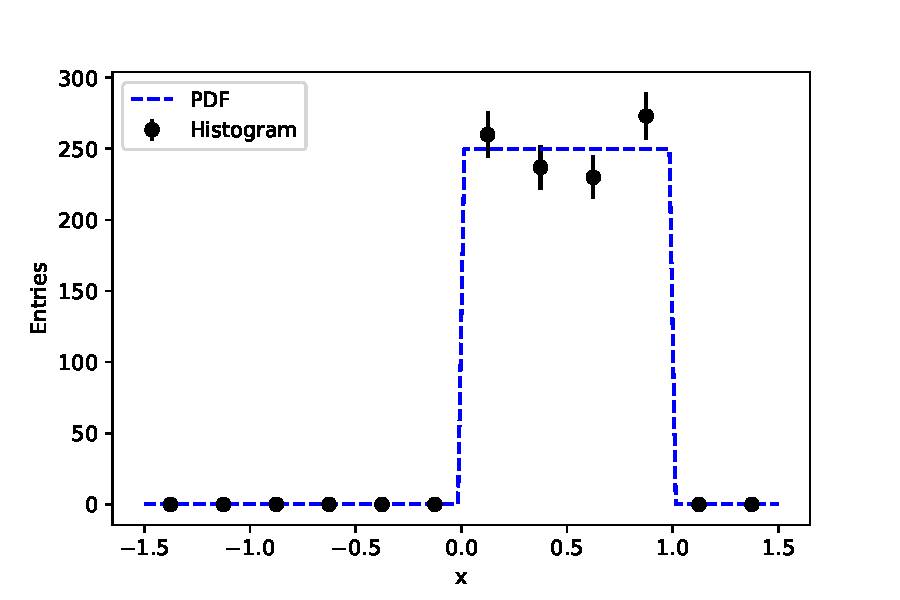
\includegraphics[width=0.45\textwidth]{figs/hist/histpdf.pdf}}
\end{center}
\caption{\label{fig:histpdf} Direct comparison of a histogram containing 1000 events thrown uniformly in the range $[0,1]$ with the corresponding PDF, scaled appropriately.}
\end{figure}

\plot Add a plot of the scaled PDF to your histogram, to produce a figure like that of Fig.~\ref{fig:histpdf}\\


\section{Calculating the value of $\pi$}

\begin{figure}[htbp]
\begin{center}

\includegraphics[width=0.65\textwidth]{figs/monte_carlo/pitoss.jpg} 
\caption{Determining $\pi$ by throwing toothpicks.}
\label{fig:pitoss}
\end{center}
\end{figure}

\noindent
You can be the life of your next party by showing off how to determine
the constant $\pi$ by throwing toothpicks!  The procedure is simple:
you cut a piece of paper to a width of four toothpicks, then draw two
vertical lines separated by the width of two tooth picks.  Take turns
tossing toothpicks, as in Fig.~\ref{fig:pitoss}.

From the geometry of the setup, it can be shown that the probability
that a toothpick which is entirely on the paper also crosses a line is
given by $1/\pi$.  Therefore, one can measure $\pi$ by counting the
total number of toothpicks that landed entirely on the page and
dividing by the number of those toothpicks that crossed a line.  This
is, in essence, the Monte Carlo method.

\begin{figure}[htbp]
\begin{center}
  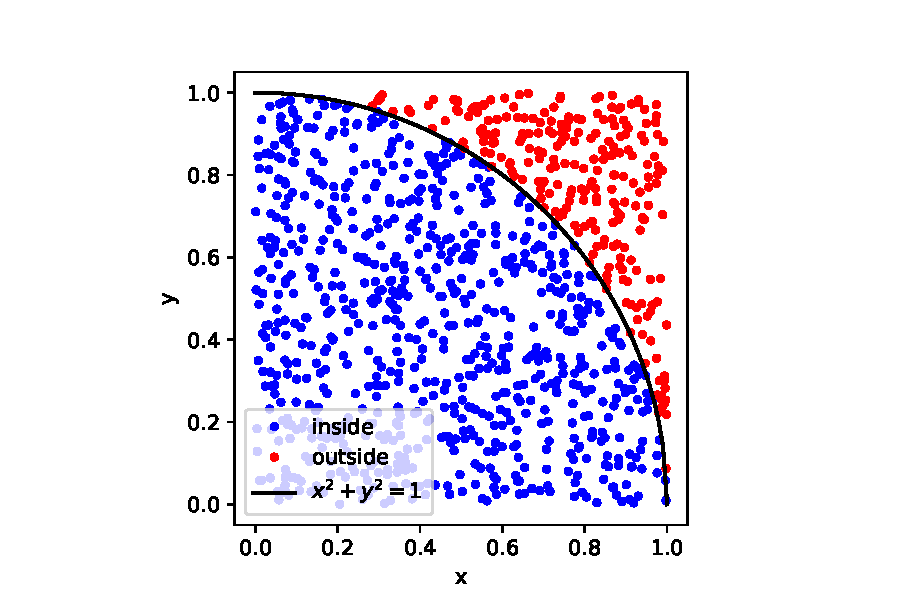
\includegraphics[width=0.9\textwidth]{figs/ideal_gas/pimc.pdf}
\caption{Monte Carlo Determination $\pi$ .}
\label{fig:pimc}
\end{center}
\end{figure}

An easier Monte Carlo method to implement computationally is 
shown in Fig.~\ref{fig:pimc} which was generated with following code:
\begin{python}
N = 1000 # number of random values to throw
# throw N x and y random variables uniform in [0,1]
x = np.random.uniform(size = N)
y = np.random.uniform(size = N)
# determine which (x,y) position or inside/outside the unit circle:
rsq = x**2 + y**2
inside  = rsq<=1
outside = np.logical_not(inside)
# set aspect ratio to 1 so unit circle looks like a circle.
plt.axes().set_aspect('equal')
# plot inside as blue dots and outside as red dots
plt.plot(x[inside],y[inside],"b.",label="inside")
plt.plot(x[outside],y[outside],"r.",label="outside")
# plot the unit circle:
xfin = np.linspace(0,1,100)
yfin = sqrt(1-xfin**2)
plt.plot(xfin,yfin,"k-",label="$x^2+y^2=1$")
# add labels and legends:
plt.xlabel("x")
plt.ylabel("y")
plt.legend(loc=3)
\end{python}
The idea is to throw points uniformly in the unit square of area 1.
Much like in the toothpick example, the value of $\pi$ can be
determined by counting the number of generated points which also
landed within the unit circle.  Make sure you understand the example
code, particular how masks are used to draw the blue and red dots.\\

\plot Run the example code.  Then, count the number of points inside the unit circle using:
\begin{python}
n_inside = np.sum(inside)
\end{python}
Estimate $\pi$ using the Monte Carlo method.  Hint: based on area, what fraction of total events do you expect to find within the unit circle?\\

\plot (Optional)  This is an example of a binomial process, and the statistical
uncertainty on your measured value of $\pi$ works out to be:
\begin{displaymath}
\sigma_\pi = \sqrt{\frac{\pi \, (4-\pi)}{n}}
\end{displaymath}
where $n$ is the number of generated events.  Does your measured value
of $\pi$ agree with the known value within your statistical
uncertainty?\\

\section{Monte Carlo integration}
\label{sec:mcint}

The Monte Carlo method can also be used to numerically integrate a
function.  Monte Carlo integration methods generally only outperform
deterministic methods when the number of dimensions is large, but we
can illustrate the method most easily in one dimension. In this
section, you'll use the Monte Carlo method to perform the integral:
\begin{displaymath}
  \int_0^\pi \sin^2 \theta \, d\theta
\end{displaymath}

To do so, you should make a copy of your solution from the previous section
and modify it in the following manner:
\begin{itemize}
 \item Instead of thowing $x$ in $[0,1]$, throw $\theta$ in $[0,\pi]$.  This means the area of the rectangle $A$ is now $\pi$ instead of 1.
 \item Count the number of throws that land below the integral $y < \sin^2 \theta$.
 \item Determine the area under the curve as the fraction of the throws under the curve times the total area of the rectangle $A$.
 \item The statistical uncertainty in this case is $\pi/(2\sqrt{n})$ where $n$ is the number of generated events.
\end{itemize}  

\begin{plot} \end{plot}
Use the Monte Carlo method to calculate the integral:
\begin{displaymath}
  \int_0^\pi \sin^2 \theta \, d\theta
\end{displaymath}
Make a plot similar to that of Fig.~\ref{fig:pimc} showing the thows
above the curve in red and below the curve in blue.  Calculate the
integral and statistical uncertainty and compare it to the value you obtain analytically.

\section{Ideal Gas in Two Dimensions}

\begin{figure}[htbp]
\begin{center}
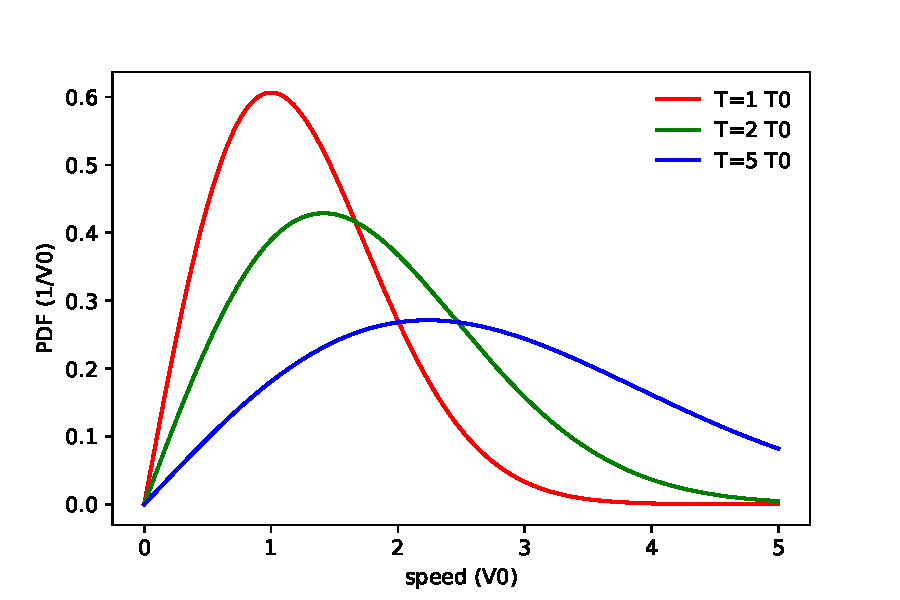
\includegraphics[width=0.65\textwidth]{figs/ideal_gas/mbspeed.pdf} \\
\caption{The Maxwell-Boltzmann distribution, for three different
  temperatures, using the system of units chosen for the numerical
  simulation.}
\label{fig:mbspeed}
\end{center}
\end{figure}

\noindent
For the remainder of this lab, we will calculate the statistical
properties of a simulated ideal gas and compare to the theoretical
prediction.  Our ideal gas will be composed of molecules with mass $m$
and held at temperature $T$.  To keep things simple, we will consider
a two dimensional gas.

A fundamental result from statistical mechanics is that the
propability of finding a single gas molecule in a state with energy
$E$ is proportional to the Boltzman factor:
\begin{displaymath}
P(E) \; \propto \; \exp\left(-\frac{E}{k_{\rm B}T}\right)
\end{displaymath}
where $k_{\rm B}$ is Boltzmann's constant.  Since the ideal gas has no
interactions, its energy is purely kinetic energy, and in two
dimensions this is given by:
\begin{displaymath}
E = \frac{1}{2} \, m \, (v_x^2 + v_y^2)
\end{displaymath}
So we can conclude:
\begin{displaymath}
P(v_x, v_y) \; \propto \; \exp\left(-\frac{m\,(v_x^2+v_y^2)}{2k_{\rm B}T}\right)
=
\exp\left(-\frac{m\,v_x^2}{2kT}\right) \cdot \exp\left(-\frac{m\,v_y^2}{2kT}\right)
\end{displaymath}
We can infer that the probability density for the component of velocity in $x$ direction is given by:
\begin{equation}
  \label{eqn:mbvx}
P(v_x) = \sqrt{\frac{m}{2 \pi k_{\rm B} T}} \exp\left(-\frac{m v_x^2}{2k_{\rm B} T}\right)
\end{equation}
where we have calculated the normalization constant such that:
\begin{equation*}
\int_{-infty}^{+\infty} P(v_x) dv_x = 1.
\end{equation*}
Similary:
\begin{equation}
  \label{eqn:mbvy}
P(v_y) = \sqrt{\frac{m}{2 \pi k_{\rm B} T}} \exp\left(-\frac{m v_y^2}{2k_{\rm B} T}\right)
\end{equation}

Now we shall find the PDF associated with a particular speed $v$.  We consider the infinitesimal probability for a particular velocity
\begin{eqnarray*}
P(v_x) P(v_y) \, dv_x \, dv_y
  &=& \frac{m}{2 \pi k_{\rm B} T} \exp\left(-\frac{m (v_x^2+v_y^2)}{2k_{\rm B} T}\right) \, dv_x \, dv_y \\
  &=& \frac{m v}{2 \pi k_{\rm B} T} \exp\left(-\frac{m v^2}{2k_{\rm B} T}\right) \, d\theta \, dv \\
\end{eqnarray*}
where we have changed to polar coordinates $v$ and $\theta$ in the usual manner with area differential $dv_x \, dv_y = v \, dv \, d\theta$.  This allows us to read off the probability density in polar coordintes:
\begin{equation*}
P(v, \theta) = \frac{m v}{2 \pi k_{\rm B} T} \exp\left(-\frac{m v^2}{2k_{\rm B} T}\right) 
\end{equation*}
Integrating over all possible directions $\theta$, we obtain:
\begin{eqnarray}
P(v) &=& \int_0^{2\pi} P(v,\theta) d\theta \nonumber \\
     &=& \int_0^{2\pi} \frac{m v}{2 \pi k_{\rm B} T} \exp\left(-\frac{m v^2}{2k_{\rm B} T}\right) \nonumber \\
P(v) &=& \frac{m v}{k_{\rm B} T} \exp \left(-\frac{m v^2}{2k_{\rm B} T}\right) \label{eqn:mbv}\\
\nonumber
\end{eqnarray}
which is the Maxwell-Boltzmann distribution for an ideal gas in two
dimensions.  This is the probability density for a gas molecule to
have speed $v$. It is illustrated in Fig.~\ref{fig:mbspeed}.  In this
lab, we will create a simple numerical simulation of an ideal gas and
verify that the velocity of the gas follows this distribution.

\section{System of Units}

Choosing an effective system of units is essential for building a
well-behaved numerical simulation.  By now you have hopefully learned
the wisdom of solving problems analytically using only variables,
plugging actual numbers into your equations only if necessary and only
at the very end.  Numerical techniques generally depend on using
actual numerical values, but by making a wise choice for a
computational system of units, we can recover the same universality
and clarity that variables provide to analytic solutions.

Consider the Maxwell-Boltzmann distribution, which involves the following SI values:
\begin{itemize}
\item Boltzmann's constant: $k_{\rm B} = 1.38 \times 10^{-23}~\rm J/K$
\item Molecular masses: e.g. $N_2$ with $m =  4.65 \times 10^{-26}~ \rm kg$.
\item Temperature: e.g. room temperature $T = 293~\rm K$.
\end{itemize}
The smallest number greater than zero that a computer can represent
with a single-precision floating point number is approximately
$10^{-38}$. Representing the SI value of Boltzmann's constant at
$10^{-23}$ uses a large fraction of this precision before we even begin
our calculation.  Numerical algorithms using floating point numbers
work best when the values involved in the calculation are near one.

It is usually best, therefore, to devise an alternate system of units
for any numerical simulation which keeps the values of variables of
interest as near one as possible.  We will call this the numerical
system of units.

To start, we choose a reference temperature near the temperature
we would like to simluate, say $T_0 = 293~\rm K$.  All temperatures in
the simulation will be in units of this reference temperature.  So a
temperature \pyth{T=1.2} in the program will be $1.2~T_0 = 352~\rm K$
in SI units.  Our model also includes mass, so we choose a reference
mass near the mass of the molecules we will be simulating, say $M_0 =
4.65 \times 10^{-26}~ \rm kg$.  A mass {\tt m=2.1} in our program would have
an SI value value of $2.1~M_0 = 9.8 \times 10^{-26}~ \rm kg$.

The physics we will simulate involves Boltzmann's constant $k_{\rm B}$
which will have a value of one in our program.  This sets the
reference energy from our reference temeperature.  For example, an
energy {kT == 3} in our program will have an SI value of $k_{\rm B}
T = 3~k_B~T_0 = 1.21 \times 10^{-20}~J$.  The reference energy and
reference mass together define a reference velocity:
\begin{displaymath}
V_0 = \sqrt{\frac{k_b T_0}{M_0}} = 295~ \rm m/s.  
\end{displaymath}  

The only time the actual values choosen for the numerical system of
units are needed is if you need to convert inputs in SI units to the
numerical system of units, or convert the results of your simulation
to SI units.  In this lab, we will specify all inputs and report all
results using the numerical system of units.  {\bf So there is no need
  for specific values such as $M_0 = 2.32 \times 10^{-25}~\rm kg$ to
  appear anywhere in your program.}  If such values do appear, outside
of comments, you are certainly making a mistake!  If you are living
entirely within the numerical system of units, there is no need to
even define $M_0$: this is how you recover universality in numerical
simulations.\\

\plot Using the numerical system of units:
\begin{python}
# computational system of units:
M  = 1 # mass of gas particles, M0 = 4.65E-26 kg
T  = 1 # Temperature of gas, T0 = 293 K
kb = 1 # Boltzmans constant
\end{python}
and the Maxwell-Boltzman distribution:
\begin{python}
  def mbspeed(v):
      return (M*v / (kb*T))*np.exp(-M*v**2/(2*kb*T))
\end{python}
plot the Maxwell-Boltzman distribution for v = 0 to $5~V_0$.  Compare with Fig.~\ref{fig:mbspeed}.\\

Notice how the relevant velocities for T=1 are near v=1.  This is sign
of good numerical system of units.  Notice also that Boltzmann's
constant or any other small or large numbers in SI units do not appear
anywhere in the code (only in comments).\\

\plot Suppose we set $M_0=10^{-15}~\rm kg$ instead.  Would your plot
in the previous exercise need to be changed?  What about
Fig.~\ref{fig:mbspeed}?  From Fig.~\ref{fig:mbspeed}, read off the
peak of the distribution for T = 2 T0.  What is that in SI units,
assuming $M_0=4.65 \times 10^{-26}~\rm kg$?  What if $M_0=10^{-15}~\rm
kg$?  Do we even need to specify $M_0$ if we do not care about the
specific SI values?  Is choosing a computational system of units with
variables near one the numerical analysis equivalent to solving a
problem using variables only?

\section{Collision Model}

At the heart of your numerical simulation is the collision model.  It
is the collisions of molecules that will allow your simulated gas to
reach thermal equilibrium.  We will use the simple elastic collision
of identical mass particles, as illustrated in Fig.~\ref{fig:collcms}, as our collision model.  We consider particles a and b with velocities $\vec{v_a}$ and
$\vec{v_b}$ in the lab frame.  The velocity of particle a in the CMS frame before the collision is
\begin{displaymath}
\vec{u} = \frac{\vec{v_a} - \vec{v_b}}{2}.
\end{displaymath}
and the velocity of particle b is $-\vec{u}$.

The collision rotates the velocity of particle a by the scattering angle $\theta$ so that the velocity $\vec{w}$ after the collision is
\begin{displaymath}
\begin{pmatrix}
w_x \\
w_y \\
\end{pmatrix}
  =
\begin{pmatrix}
\cos \theta  & -\sin \theta \\
\sin \theta  & \cos \theta \\
\end{pmatrix}
\,
\begin{pmatrix}
u_x \\
u_y \\
\end{pmatrix}
\end{displaymath}
The velocity of particle b after scattering is $-\vec{w}$.

In the lab frame, the velocity of molecule a changes by an amount:
\begin{displaymath}
\Delta \vec{v_a} = \vec{w} - \vec{u}  
\end{displaymath}
and the velocity of molecule b changes by an amount:
\begin{displaymath}
\Delta \vec{v_b} = (-\vec{w}) - (-\vec{u}) = -\Delta \vec{v_a}
\end{displaymath}

\begin{figure}[htbp]
\begin{center}
\begin{tikzpicture}
\draw[->, line width=1.5, blue] (-3,0) -- (-0.1,0);
\draw[->, line width=1.5, blue] (3,0)  -- (0.1,0);
\draw[->, line width=1.5, red] (0,0) -- (3*0.50,3*0.86) coordinate(A);
\draw[->, line width=1.5, red] (0,0) -- (-3*0.50,-3*0.86) coordinate(B);
\node[right] at (0.5,0.5) {$\theta$};
\node[left] at (-3,0) {a};
\node[right] at (3,0) {b};
\node[above] at (A) {a};
\node[below] at (B) {b};
\node[above] at (-1.5,0) {$\vec{u}$};
\node[above] at (1.5,0) {$-\vec{u}$};
\node[left] at (0.8,1.5) {$\vec{w}$};
\node[left] at (-0.8,-1.4) {$-\vec{w}$};
\end{tikzpicture}
\caption{The collision model in the center-of-mass:  incoming molecule $a$ with velocity $\vec{u}$ collides with the incoming particle $b$ of identical mass with velocity $-\vec{u}$.  Particle $a$ is scattered by angle $\theta$ and leaves with velocity $\vec{w}$, while particle $b$ leaves with velocity $\vec{w}$.  The magnitude of the final and initial velocities are the same:  $|\vec{u}| = |\vec{w}|$.}
\label{fig:collcms}
\end{center}
\end{figure}

\section{Implementing the Collision Model}

Our Python implementation for the collision will be computed in terms
of the components of the velocity vectors of molecule a and molecule
b:
\begin{eqnarray*}
\vec{v_a} &=& 
\begin{pmatrix}
a_x \\
a_y \\
\end{pmatrix} \\
\vec{v_b} &=& 
\begin{pmatrix}
b_x \\
b_y \\
\end{pmatrix} \\
\end{eqnarray*}
We'll use the Python variable names {\tt ax}, {\tt ay}, {\tt bx}, and {\tt by} to refer to $a_x$,  $a_y$,  $b_x$, and $b_y$.  

First calculate the $x$ and $y$ component of $\vec{u}$ as:
\begin{eqnarray*}
u_x &\equiv& \frac{a_x - b_x}{2} \\
u_y &\equiv& \frac{a_y - b_y}{2} \\
\end{eqnarray*}
Then compute the $x$ and $y$ component to the change in velocity of particle a and particle b:
\begin{eqnarray*}
  \Delta a_x &=& (\cos\theta - 1) \, u_x - \sin\theta \, u_y \\
  \Delta a_y &=& (\cos\theta - 1) \, u_y + \sin\theta \,  u_x \\
\end{eqnarray*}
Finally, update the $x$ and $y$ components of the particle velocities to their value after the collision:
\begin{eqnarray*}
  a_x &\to& a_x + \Delta a_x \\
  a_y &\to& a_y + \Delta a_y \\
  b_x &\to& b_x - \Delta a_x \\
  b_y &\to& b_y - \Delta a_y \\
\end{eqnarray*}

\newpage

\plot Implement the collision model as a Python function:
\begin{python}
def collide(ax,ay,bx,by,theta):
    # your code here
    return ax, ay, bx, by # updated values
\end{python}
which takes the lab frame veclocitys of particle a (ax,ay) and b (bx, by) and returns the lab frame velocities after scattering by an angle theta.  Test your code with some simple cases first, rotations by zero,quarter,half,and three quarters of a full turn:
\begin{python}
tau = 2*np.pi # Using 2 pi is like saying twice half-way...
# lab frame is cms, incoming on x axis:
print(np.around(collide(1,0,-1,0,0),2)+0)
print(np.around(collide(1,0,-1,0,tau/4),2)+0)
print(np.around(collide(1,0,-1,0,tau/2),2)+0)
print(np.around(collide(1,0,-1,0,3*tau/4),2)+0)
\end{python}
which should have the output:
\begin{verbatim}
[ 1.  0. -1.  0.]
[ 0.  1.  0. -1.]
[-1.  0.  1.  0.]
[ 0. -1.  0.  1.]
\end{verbatim}
And:
\begin{python}
# lab frame is cms, incoming on	y axis:
print(np.around(collide(0,1,0,-1,0),2)+0)
print(np.around(collide(0,1,0,-1,tau/4),2)+0)
print(np.around(collide(0,1,0,-1,tau/2),2)+0)
print(np.around(collide(0,1,0,-1,3*tau/4),2)+0)
\end{python}
which should have the output:
\begin{verbatim}
[ 0.  1.  0. -1.]
[-1.  0.  1.  0.]
[ 0. -1.  0.  1.]
[ 1.  0. -1.  0.]
\end{verbatim}

\newpage

When debugging code, start with simple test cases.  If you get the
wrong answer, it will be easy to see where the calculation is going
wrong.  Once your code works on the simple tests cases, start adding
more complexity:\\

\plot Test your collision function where the lab frame is not the CMS frame:
\begin{python}
# boost along x axis, incoming on y axis:
print(np.around(collide(1,1,1,-1,0),2)+0)
print(np.around(collide(1,1,1,-1,tau/4),2)+0)
print(np.around(collide(1,1,1,-1,tau/2),2)+0)
print(np.around(collide(1,1,1,-1,3*tau/4),2)+0)
\end{python}
which should output:
\begin{verbatim}
[ 1.  1.  1. -1.]
[0. 0. 2. 0.]
[ 1. -1.  1.  1.]
[2. 0. 0. 0.]
\end{verbatim} \vskip 0.25cm

\plot Test your collision function with randomly choosen values:
\begin{python}
# test with random values:
print(np.around(collide(6.24, 1.78, 3.35, 5.98, 3.19),2))
print(np.around(collide(4.07, 4.69, 1.61, 4.54, 2.46),2))
print(np.around(collide(5.28, 2.99, 4.77, 5.22, 3.15),2))
print(np.around(collide(2.84, 5.37, 5.47, 6.16, 1.59),2))
\end{python}
which should output:
\begin{verbatim}
[3.25 5.91 6.34 1.85]
[1.84 5.33 3.84 3.9 ]
[4.76 5.22 5.29 2.99]
[4.58 4.46 3.73 7.07]
\end{verbatim}

\section{Initializing the Simulated Ideal Gas}

We will be modeling an ideal gas by direct Monte Carlo simulation of
\pyth{NGAS} representative molecules.  The state of your simulation
will be completely contained in two numpy arrays {\tt vx} and {\tt
  vy}, each of length {\tt NGAS}, which contain the velocities of the
particles in units of $V_0 = \sqrt{k_b T_0 / M_0}$.  Remember, the
simulation uses a system of units that should keep velocities near 1,
so values such as 2.2, -3.1, 0.8, -0.01 are all likely, and correspond
to speeds of up to several hundred meters per second in SI units.  On
the other hand, the presence of extremely small values, like 5.3E-23,
and extremely large values like 1.2E18 and -8.2E28 are symptoms of
bugs.\\

\plot Start with a small number of molecules \pyth{NGAS=5}.  Use the
\pyth{np.random.uniform} function to initialize the \pyth{vx} and
\pyth{vy} arrays with random values choosen uniformly in the range
(-2,2).  Print your arrays and see if the output is reasonable.\\

Our simulation is going to grow to contain at least 1000 molecules, so
printing the values of each molecule is not going to work.  So we will want to visualize it as a histogram.\\

\plot Increase NGAS to 1000, and plot the $v_x$ array as a histogram:
\begin{python}
hvx,bins = histogram(vx,bins=20,range=(-5,5))
cbins = (bins[1:]+bins[:-1])/2
plt.errorbar(cbins,hvx,yerr=np.sqrt(hvx),fmt="o")
\end{python}
~\\ \vskip -0.5cm

\plot Plot the $v_y$ distribution as a histogram.\\

Your histograms should reveal that your distribution of velocities is
flat, just like in Fig.~\ref{fig:histpdf}.  The gas molecules have not
yet reached thermal equilibrium with each other!

\section{Collisions of an Ideal Gas}

To reach thermal equilibrium, you'll need to simulate collisions
betweens pairs of molecules in your gas.  For each collision, do the following:
\begin{itemize}
 \item Choose two molecules at random as particles $a$ and $b$. (See {\tt np.random.choice}.)
 \item Choose a random value $\theta$ uniformly in the range $[0,2\pi]$ (See {\tt np.random.uniform}.)
 \item Call your collision function with components of the velocity vectors for particles $a$ and $b$ and the scattering angle $\theta$.
 \item Update the velocity of particles $a$ and $b$ from the return value of your collision funciton
\end{itemize}   
For this model, you will need about 10 times as many collisions as gas
molecules in order to reach thermal equilibrium.\\

\plot For \pyth{NGAS=1000} moleculres, simulated \pyth{NCOLL=10000}
collisions using the algorithm described above.  Plot the vx and vy
distributions as a histogram:
\begin{python}
hvx,bins = histogram(vx,bins=20,range=(-5,5))
hvy,bins = histogram(vy,bins=20,range=(-5,5))
cbins = (bins[1:]+bins[:-1])/2
plt.errorbar(cbins,hvx,yerr=np.sqrt(hvx),fmt="bo",label="vx")
plt.errorbar(cbins,hvy,yerr=np.sqrt(hvx),fmt="ro",label="vy")
plt.xlabel("Velocity (V0)")
plt.ylabel("Molecules")
plt.legend()
\end{python}

\section{Temperature of an Ideal Gas}

The temperature of the gas is related to the mean kinetic energy by:
\begin{equation}
\label{eqn:kt}
k_b T = m \, \frac{\braket{v_x^2} + \braket{v_y^2}}{2}  
\end{equation}  
You can estimate $\braket{v_x^2}$ from your simulation as {\tt np.mean(vx**2)}.\\

\plot Estimate $kT$ of the gas using Equation~\ref{eqn:kt} before and after simulating collisions.
The values should remain near the expected value 4/3.


\section{The Maxwell-Boltzmann Distribution}
\label{sec:mbdist}


In this section, you'll reproduce the instructor plots of
Fig.~\ref{fig:mbinst} using your own numerical simulation.\\

\begin{figure}[htbp]
\begin{center}
  \begin{tabular}{cc}   
  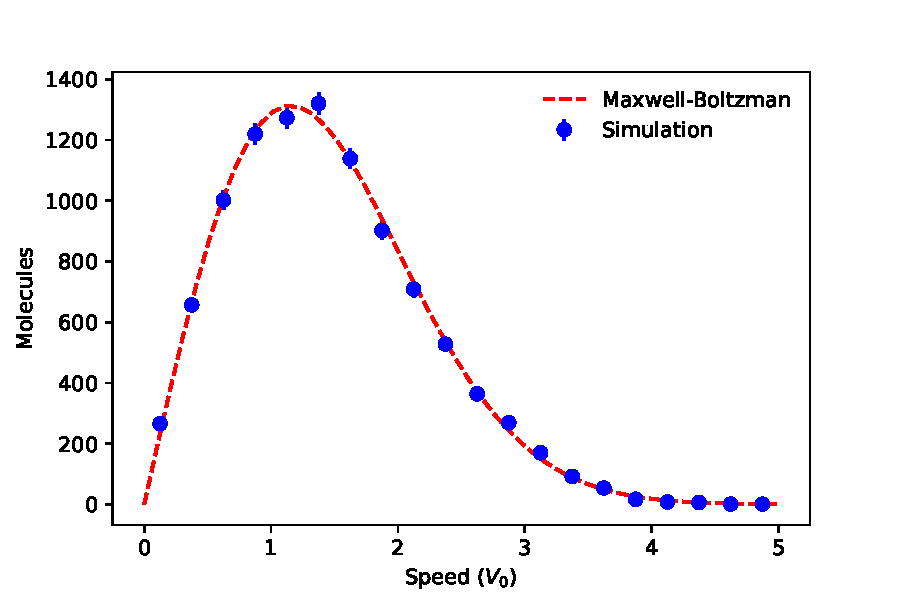
\includegraphics[width=0.45\textwidth]{figs/maxwellboltzman/mbinstv.pdf} &
  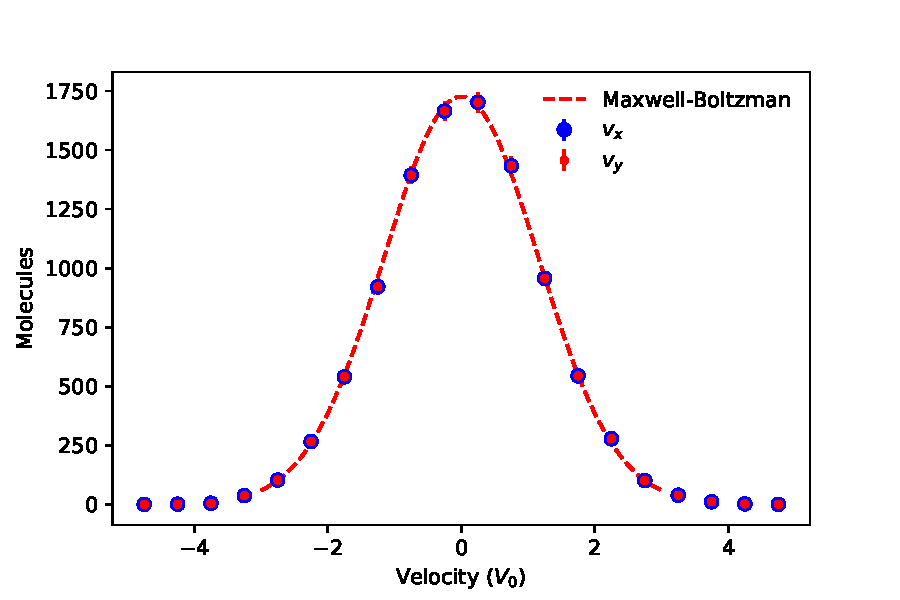
\includegraphics[width=0.45\textwidth]{figs/maxwellboltzman/mbinstvxvy.pdf} \\
  (a) & (b) \\
  \end{tabular}
\caption{Instructor plots.}
\label{fig:mbinst}
\end{center}
\end{figure}

\plot After your simulation reaches equilibrium, plot two histograms,
one with $v_x$ and one with $v_y$, with an approriate range and 10
bins.  Directly compare your histograms with the PDF from
Equation~\ref{eqn:mbvx}, scaled appropriately.  The results should
resemble the right side of Fig.~\ref{fig:mbinst}, which were produced
with {\tt NGAS=10000}.\\

\plot After your simulation reaches equilibrium, fill a histograms
with the magnitude of the velocity $v$, with an approriate range and
10 bins.  Compare with the prediction from Equation~\ref{eqn:mbv}.
The results should resemble the left side of Fig.~\ref{fig:mbinst},
which were produced with {\tt NGAS=10000}.\\

\section{Ideal Gas Law}
\label{sec:idealgas}

This section contains only optional challenge problems.  Only minimal
instructor help will be available for these problems.\\

\plot (Optional Challenge) Implement a function which scales the
velocities $v_x$ and $v_y$ by an appropriately choosen factor to set
the temperature of the gas to any desired temperature $T$.  Set the
temperature to $1~T_0$, and show that the gas follows the
Maxwell-Boltzman distribution for $T=1~T_0$.\\

The ideal gas law for a 2-D gas of $N$ molecules at temperature $T$ is
\begin{displaymath}
  Q A = N \, k_{\rm b} T
\end{displaymath}
where $Q$ is the 2-D analog for pressure: a force per unit distance.
We'll consider a rectangular region of gas with height $H$ and length
$L$.  In this case, the ideal gas law becomes:
\begin{displaymath}
  F L = N \, k_{\rm b} T
\end{displaymath}
where $F$ is the total outward force acting on a each boundary of height $H$.

Our computational system of units will be extended to include a
distance $L_0$.  As long as we don't need to convert to SI units,
there is no need for us to specify $L_0$ in meters.  The units of time
are $L_0/V_0$.  The time it takes for a molecule to travel a distance
$L$ is approximately $1~L_0/V_0$, so we will step our simulation in
steps of about $\tau=0.01~L_0/V_0$.

To model the ideal gas law, we will extend our simulation to include
the $x$-position of the gas molecules.  To keep things simple, we will
simulate the motion along the $x$-axis after we have simulated
collisions and reached thermal equilibrium.

Start by generating \pyth{NGAS} $x$-positions uniformly from 0 to $L$.
Set the total momentum transferred ($\Delta p$) to zero.  During each time step,
update each $x$ value to $x + \tau \, v_x$.  For each molecule outside
the boundaries:
\begin{itemize}
 \item For $x<0$ set $x \to -x$
 \item For $x>L$ set $x \to 2L-x$
 \item Or handle both cases at once with:  $x \to (2L-x) \bmod L$
 \item Add $2 M |p_x|$ to the total momentum transferred $\Delta p$
 \item Set $v_x \to -v_x$ 
\end{itemize}   
After $N$ time steps of size $\tau$, the average force on each wall wil be given by:
\begin{displaymath}
F = \frac{\Delta p}{2 N \tau}
\end{displaymath}
If you use boolean masks effectively, you can implement this algorithm
with only a single for loop, which is needed to apply the $N$ time
steps.\\

\plot (Optional Challenge) Calculate the outward force on the wall of
the container for $L = 1 L_0$ and $T = 1 T_0$.  Compare to what you
expect from the ideal gas law.\\

\plot (Optional Challenge) Perform your Fource calculation {\em
  before} the gas reaches thermal equilirium.  Does the ideal gas law
require that the gas has reached thermal equilibrium?\\

\plot (Optional Challenge) Plot the simulated outward force on the
wall of container for several different $L$ values.  On the same axis,
plot the expected force as a function of $L$ as well.\\

\plot (Optional Challenge) Plot the simulated outward force on the
wall of container for several different $T$ values.  On the same axis,
plot the expected force as a function of $T$ as well.\\

